\graphicspath{{chapt_dutch/}{intro/}{chapt2/}{chapt3/}{chapt4/}{chapt5/}{chapt6/}{chapt7/}}

% Header
\renewcommand\evenpagerightmark{{\scshape\small Appendix A}}
\renewcommand\oddpageleftmark{{\scshape\small A data acquisition software for VME CAEN TDCs}}

\renewcommand{\bibname}{References}

\hyphenation{}

\chapter[A data acquisition software for CAEN VME TDCs]%
{A data acquisition software for CAEN VME TDCs}
\label{app1}

Certifying detectors in the perspective of HL-LHC required to develop tools for the GIF++ experiment. Among them was the \acf{DAQ} software that allows to make the communications in between the computer and the TDC modules in order to retrieve the RPC data~\cite{GIFDAQ}. In this appendix, details about the software, as of how the software was written, how it functions and how it can be exported to another similar setup.

\section{Description of the setup}
\label{app1:sec:setup}

    The CMS RPC setup at GIF++ counts 5 V1190A \acf{TDC} manufactured by CAEN~\cite{V1190AMUT}. The communication between the computer and the TDCs to transfer data is done via a V1718 VME master module also manufactured by CAEN and operated from a USB port~\cite{V1718MUT}. These VME modules are hosted into a 6U VME 6021 powered crate manufactured by W-Ie-Ne-R than can accomodate up to 21 VME bus cards~\cite{6U6000MUT}. These 3 components of the DAQ setup are shown in Figure~\ref{fig:DAQSetup}.
    
    \begin{figure}[H]
        \begin{subfigure}{0.5\linewidth}
		    \centering
			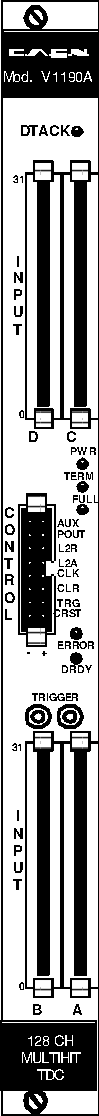
\includegraphics[height = 12cm]{fig/app1/V1190A-front.pdf}
			\caption{\label{fig:DAQSetup:A}}
		\end{subfigure}
		\begin{subfigure}{0.5\linewidth}
		    \centering
			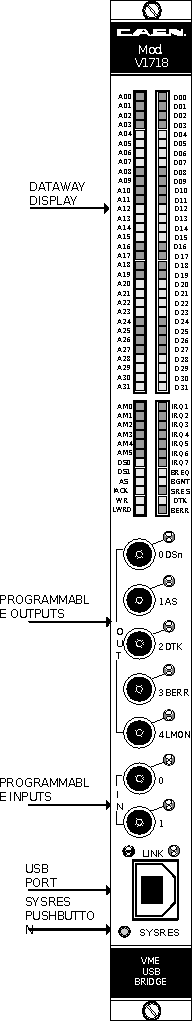
\includegraphics[height = 12cm]{fig/app1/V1718-front.pdf}\\
			\caption{\label{fig:DAQSetup:B}}
		\end{subfigure}
		\begin{subfigure}{\linewidth}
		    \centering
			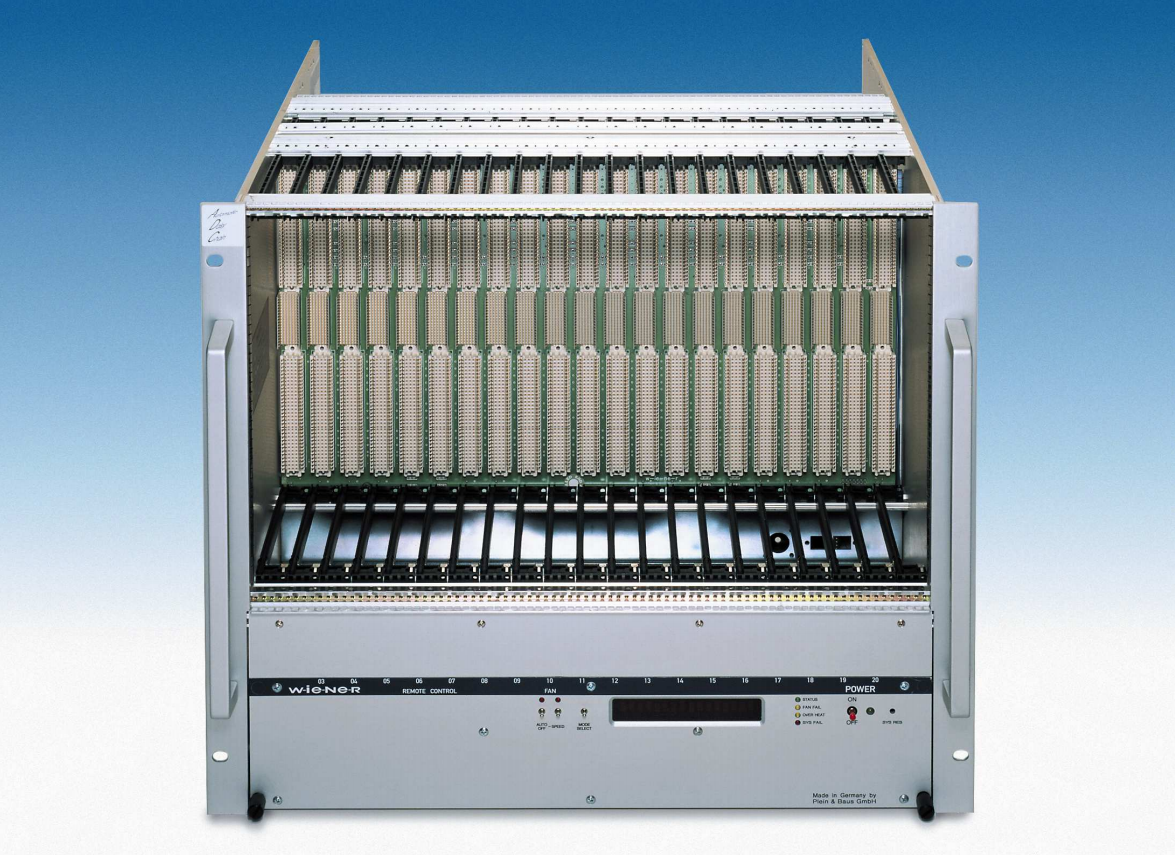
\includegraphics[width = 0.8\plotwidth]{fig/app1/Wiener-front.png}
			\caption{\label{fig:DAQSetup:C}}
		\end{subfigure}
		\caption{\label{fig:DAQSetup} (\ref{fig:DAQSetup:A}) View of the front panel of a V1190A TDC module~\cite{V1190AMUT}. (\ref{fig:DAQSetup:B}) View of the front panel of a V1718 Bridge module~\cite{V1718MUT}. (\ref{fig:DAQSetup:C}) View of the front panel of a 6U 6021 VME crate~\cite{6U6000MUT}.}
	\end{figure}

\section{Data read-out}
\label{app1:sec:Data}

    \subsection{TDC settings}
    \label{app1:ssec:TDC}

	The DAQ used at GIF takes profit of the \textit{Trigger Matching Mode} offered by V1190A modules. A trigger matching is performed in between a trigger time tag and the channel time measurements. Control over this data acquisition mode, explained through Figure~\ref{fig:V1190A-TMM}, is offered through 4 programmable parameters:
        
	\begin{itemize}
		\item \textbf{match window:} the match between a trigger and a hit is done within a programmable time window
		\item \textbf{window offset:} temporal distance between the trigger tag and the start of the trigger matching window
		\item \textbf{extra search margin:} an extended time window is used to ensure that all matching hits are found
		\item \textbf{reject margin:} older hits are automatically rejected to preven buffer overflows and to speed up the search time
	\end{itemize}
    
    \begin{figure}[H]
		\centering
		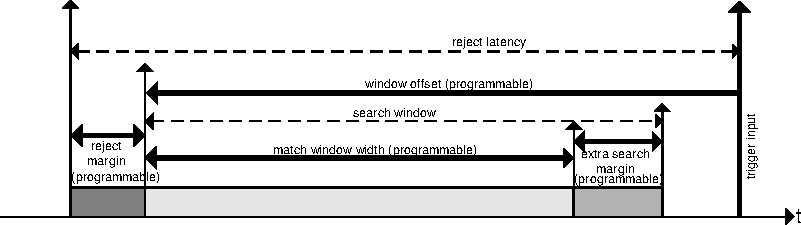
\includegraphics[width = 1.25\plotwidth]{fig/app1/V1190A-TMM.pdf}\\
		\caption{\label{fig:V1190A-TMM} Module V1190A \textit{Trigger Matching Mode} timing diagram~\cite{V1190AMUT}.}
	\end{figure}
	
	Each of these 4 parameters are given in number of clocks, \SI{1}{clock} being \SI{25}{ns} long. It is easy to understand at this level that there are 3 possible functionning settings:
        
	\begin{itemize}
		\item \textbf{1:} the match window is entirely contained after the trigger signal,
		\item \textbf{2:} the match window overlaps the trigger signal, or
		\item \textbf{3:} the match window is entirely contained before the trigger signal as displayed on Figure~\ref{fig:V1190A-TMM}.
	\end{itemize}
	
	In both the first and second cases, the sum of the window width of of the offset can be set at maximum to be \SI{40}{clocks}, which corresponds to \SI{1}{\micro s}. Of course, the offset can be negative thus allowing for a longer match window, its end being at maximum \SI{1}{\micro s} after the trigger signal. In the third case, the maximum negative offset allowed is of \SI{2048}{clocks} (12 bit) corresponding to \SI{51.2}{\micro s}, the match window being strictly smaller than the offset. In the case of GIF++, the choice has been made to use this last setting by delaying the trigger signal. During the studies performed in GIF++, both the efficiency of the RPCs, using a muon beam, and the noise or gamma background rate are monitored.\\
	To probe the efficiency of RPC detectors, a signal provided by the coïncidence of scintillators when a bunch of muons passes though the area is used to trigger the data acquisition. For this measurement, it is useful to reduce the match window width only to contain the muon information. Indeed, the delay in between a trigger signal and the detection of the corresponding muon in the RPC being very contant (typically a few tens of ns due to jitter and cable length), the muon signals are very localised in time. Thus the settings where chosen to have a window width of \SI{24}{clocks} (\SI{600}{ns}) and a negative offset of \SI{29}{clocks}.\\
	On the otherhand, monitoring the rates doesn't require for the DAQ to look at a specific time window. It is important to integrate as much time as possible to have a robust measurement of the rate as the number of hits per time unit. The triggerring signal is provided by a pulse generator at a frequency of \SI{300}{Hz} to ensure that the data taking occurs in a random way to probe only the irradiation spectrum on the detectors. The match window is set to \SI{400}{clocks} (\SI{10}{\micro s}) and the negative offset to \SI{401}{clocks} as it needs to exceed the value of the match window.\\
	
	\subsection{Data tranfer and file structure}
	\label{app1:ssec:BLT}
	
	As previously described in Section~\ref{ssec:PulseProc}, CMS RPC FEEs provide us with \SI{100}{ns} long LVDS output signals that are injected into the TDCs' input. V1190A are VME units accepting 128 independent Multi-Hit/Multi-Event TDC channels whose signals are treated by 4 \SI{100}{ps} high performance TDC chips developped by CERN / ECP-MIC Division. Any avalanche signal that gives a signal above the FEEs threshold is thus recorded by the TDCs as a hit within the match window. Each hit is assigned to a specific TDC channel with a time stamp with a precision of \SI{100}{ps}. The reference time, the 0, is provided by the beginning of the match window. thus for each trigger, coming from a scintillator coïncidence or the pulse generator, a list of hits is stored into the TDCs buffers and will then be transfered into a ROOT Tree.\\
	
	The data transfer is done via \acf{BLT}. Using BLT allows to tranfer a fixed number of events called a \textit{block}. This is used together with an \acf{AFL} of the TDCs' output buffers. This AFL gives the maximum amount of 32 bits words that can writen in the buffer before an \acf{IRQ} is generated and seen by the VME Bridge, stopping the data acquisition to transfer the content of each TDC buffers before resuming. The AFL can, at maximum, be of 32735 words (16 bits). This number corresponds to the depth of the output buffer of a TDC. For each trigger, words are written into the TDC buffer:
	
	\begin{itemize}
		\item \textbf{a global header} providing information of the event number since the beginning of the data acquisition,
		\item \textbf{a TDC header},
		\item \textbf{the TDC data}, 1 for each hit recorded during the event, providing the channel and the time stamp associated to the hit,
		\item \textbf{a TDC error} providing error flags,
		\item \textbf{a TDC trailer},
		\item \textbf{a global trigger time tag} (if enabled) that provides the absolute trigger time relatively to the last reset, and
		\item \textbf{a global trailer} providing the total word count in the event.
	\end{itemize}

\section{Software export}


\clearpage{\pagestyle{empty}\cleardoublepage}
